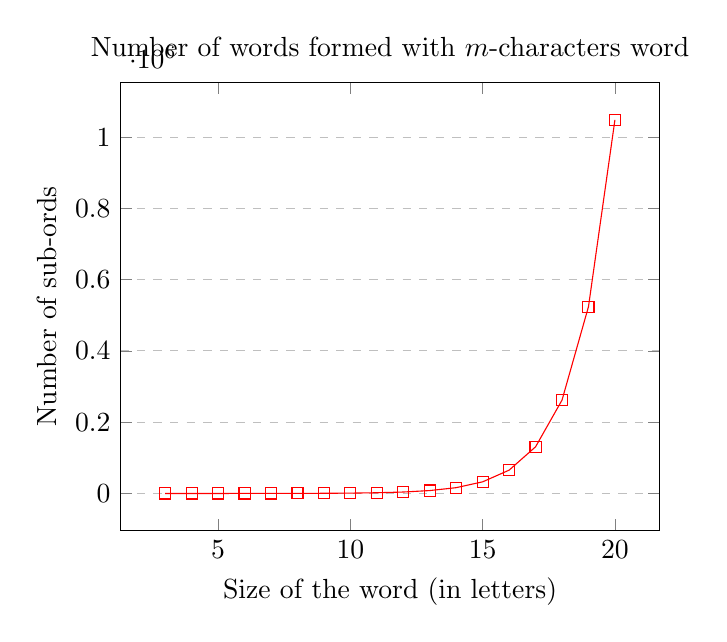
\begin{tikzpicture}
\begin{axis}[
    title={Number of words formed with $m$-characters word},
    xlabel={Size of the word (in letters)},
    ylabel={Number of sub-ords},
    % xmin=0, xmax=100,
    % ymin=0, ymax=120,
    % xtick={0,20,40,60,80,100},
    % ytick={0,20,40,60,80,100,120},
    legend pos=north west,
    ymajorgrids=true,
    grid style=dashed,
]

\addplot[
    color=red,
    mark=square,
    ]
    coordinates {
        (3, 0)
        (4, 4)
        (5, 15)
        (6, 41)
        (7, 98)
        (8, 218)
        (9, 465)
        (10, 967)
        (11, 1980)
        (12, 4016)
        (13, 8099)
        (14, 16277)
        (15, 32646)
        (16, 65398)
        (17, 130917)
        (18, 261971)
        (19, 524096)
        (20, 1048364)
    };
    
\end{axis}
\end{tikzpicture}
